\chapter{Results}
%Plan
In this chapter we showcase a series of results from the {\sc meqsilhouette} simulator. We begin with canonical simulations from the ISM, atmospheric and pointing error modules. Following this, we present the result of a typical calibration and imaging procedure in the presence of a variable source and a variable troposphere.


\section{Canonical simulations}\label{sec:can_sim}

\subsubsection{ISM variability and substructure}
%st 1

``To demonstrate the implementation and provide an example of intraday ISM variability, we present the results of a simulated observation of 10 minutes duration at 14:00 UTC on four consecutive days in Fig.~\ref{ISM_sequence}. To compare to published observations, we use the three-station EHT array consisting of the Submillimeter Telescope (SMT) in Arizona, the Combined Array for Research in Millimeter-wave Astronomy (CARMA) in California and the James Clerk Maxwell Telescope (JCMT) on Mauna Kea, Hawaii. The relative transverse velocity between the observer and scattering screen is set to $50~\rm{km\,s}^{-1}$ to be consistent with \citet{Ortiz_2016}. The source is a circular Gaussian with a $\rm{FHWM}=40$~$\mu$-arcsec, approximately the angular distance that a scattering screen would travel over $\sim 4$~days. The source size has been chosen such that it is consistent with the latest estimate of the size of Sgr~A$^\star$ at $230$~GHz \citep{Fish_2011}.  Closure quantities are model dependent and calculated as specified in \citet{Rogers_1995}, where the thermal noise was added based on the system equivalent flux density (SEFD) table in \citep{Lu_2014}.''\citep{Blecher_2016} 


\begin{figure}[h!]
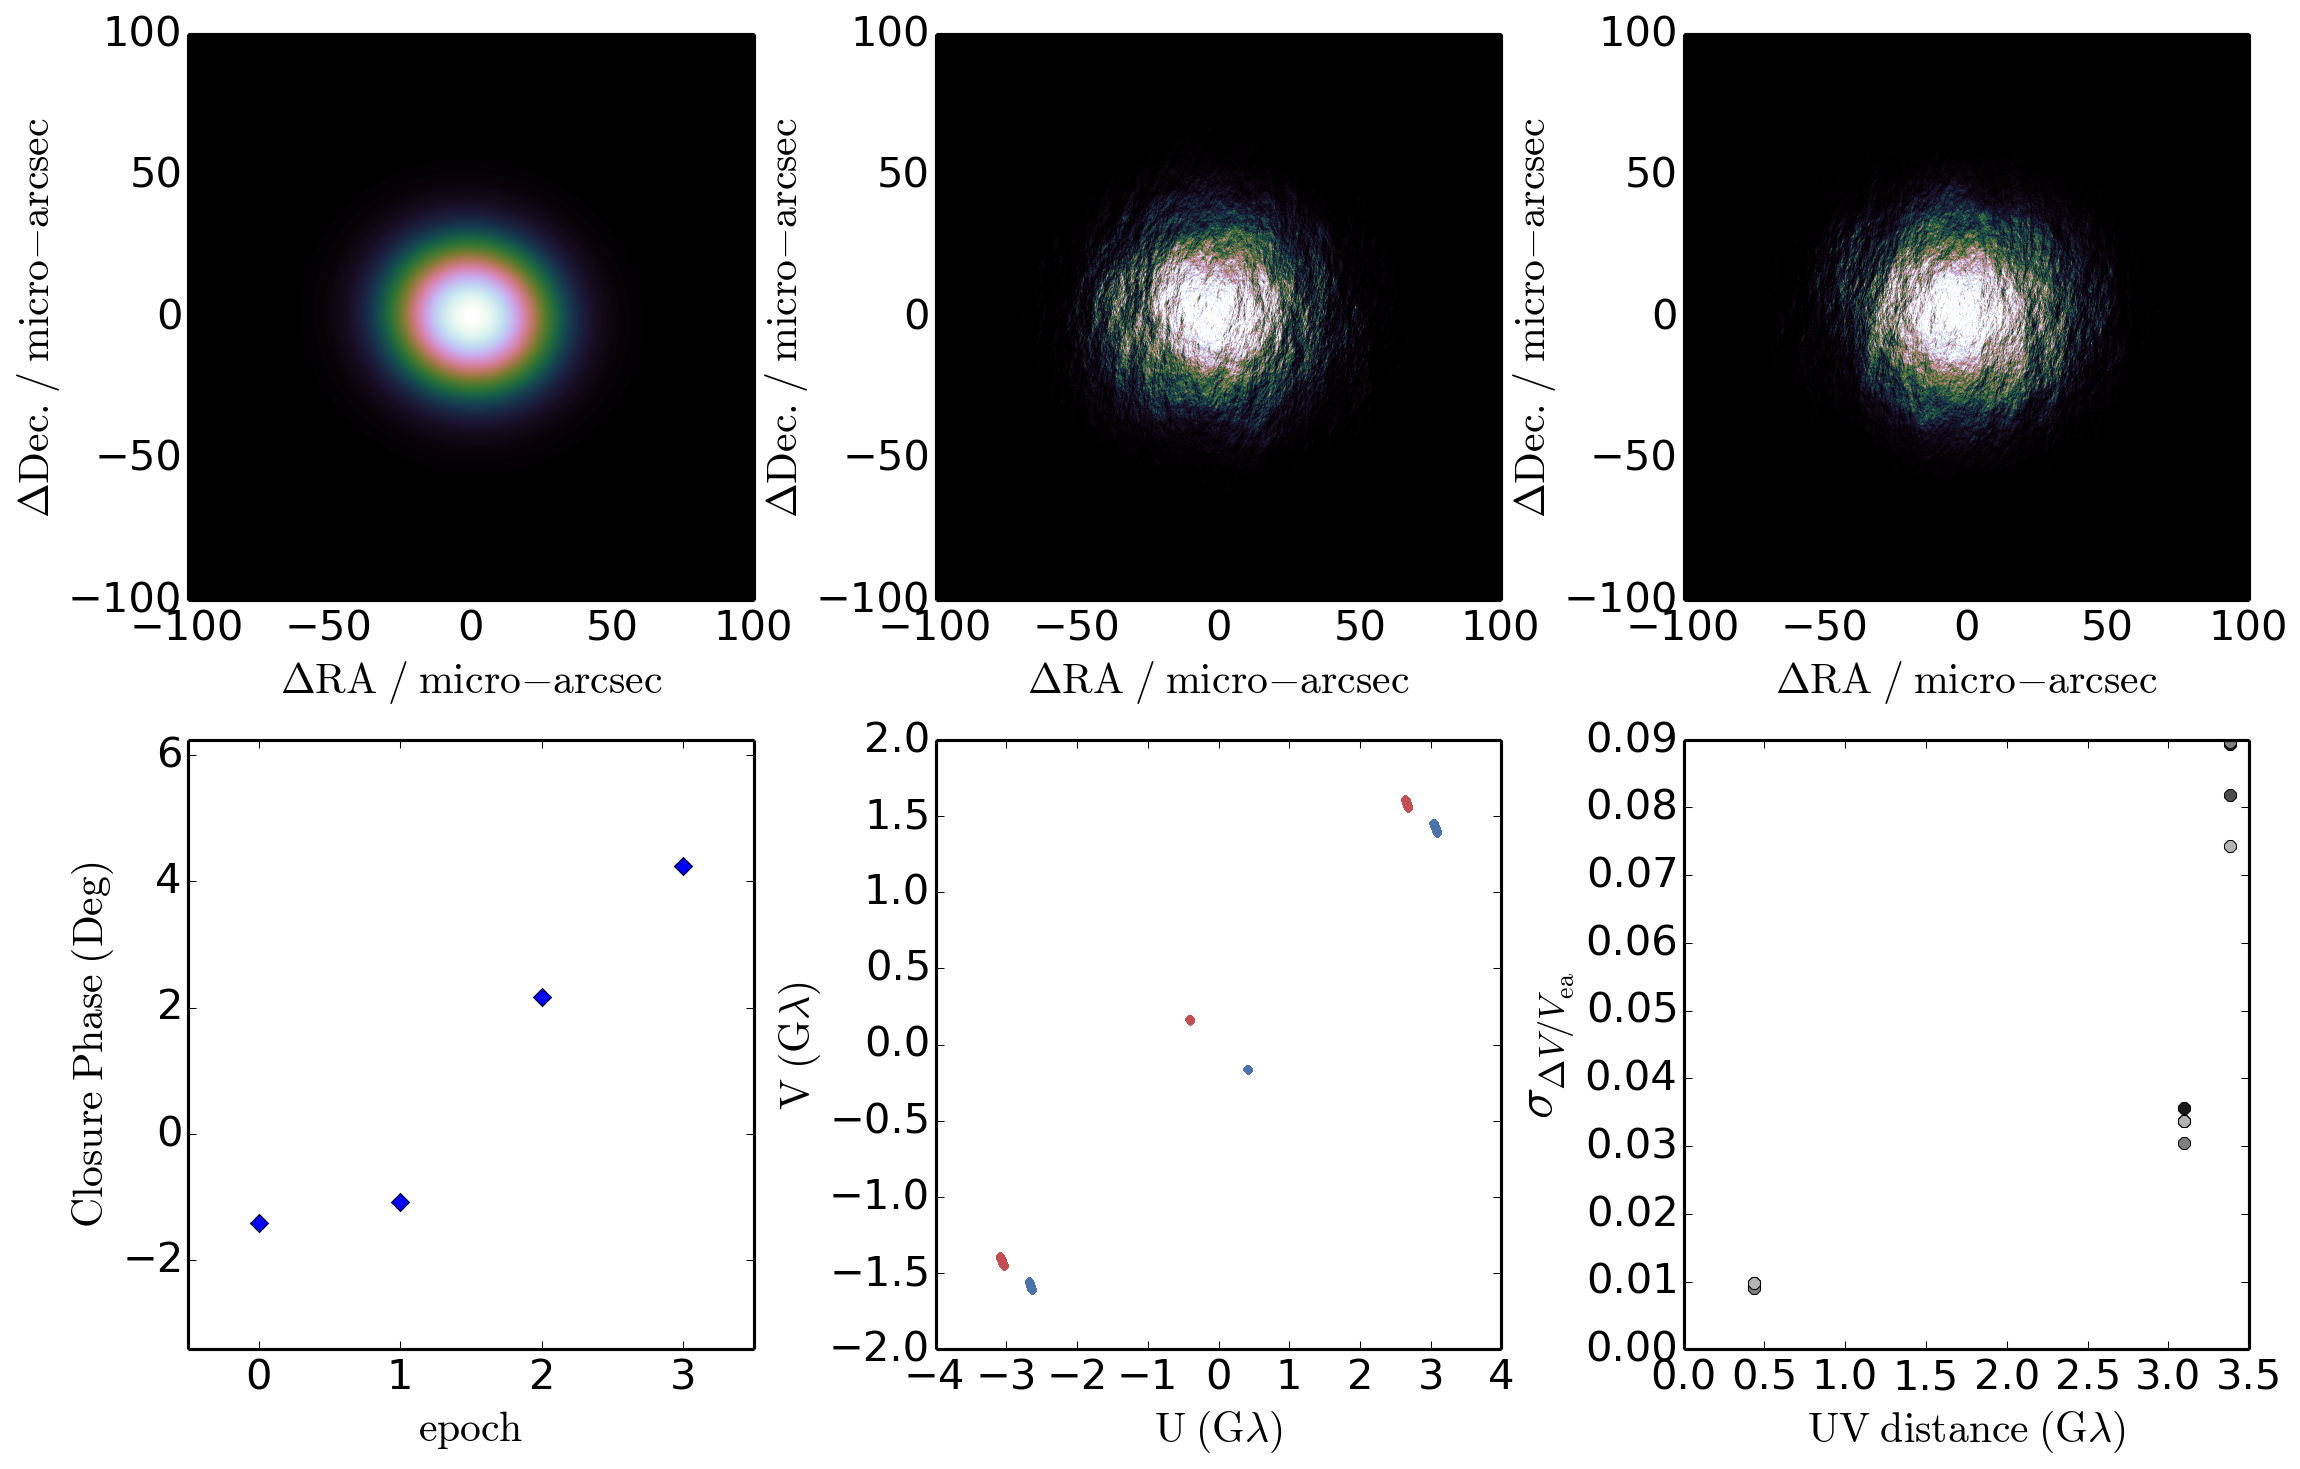
\includegraphics[width=\columnwidth]{Images/ism}
\caption{``An example simulation of ISM scattering towards Sgr~A$^{\star}$, observed with SMT-JCMT-CARMA.  The top panel, left to right, shows the original $\rm FWHM = 40$~$\mu$-arcsec Gaussian {\bf (top left)}, the simulated ISM scattered image on the first night {\bf (top middle)} and last night {\bf (top right)} of the observation, respectively.  The bottom panel, left to right,  shows the evolution of the 10 minute-averaged closure phase with epoch {\bf (bottom left)}, {\sl uv}-tracks for each night {\bf (bottom middle)} and the RMS fractional visibility amplitude differences $\sigma_{\Delta V /V_{\rm ea}}$ as a function of {\sl uv-}distance {\bf (bottom right)}. $ \Delta V= (|V_{\rm a}|-|V_{\rm ea}|)$, where $|V_{\rm a}|$ and |$|V_{\rm ea}|$ are the simulated average and ensemble average visibility amplitudes respectively. Variations from the ensemble-average flux on the shortest baselines reveal total flux modulation while flux variations on longer baselines and non-zero closure phases track the fluctuations in substructure.''(Image and text reproduced from \citet{Blecher_2016}) \label{ISM_sequence}%
}
\end{figure}


\subsubsection{Atmospheric transmission and scattering}

As laid out in section~\ref{sec:trop_imp}, our tropospheric module is separated into mean and turbulent components with the primary observables being opacity, sky brightness temperature and time delay. 
%Opacity + Brightness temperature
The first atmospheric result we present is a plot of typical opacities and sky brightness temperatures for ALMA, the Submillimeter Array (SMA) and the South Pole Telescope (SPT), shown in Fig.~\ref{fig:mean_atm}. Note that both the opacity and brightness temperature are proportional to ground pressure and inversely proportional to the ground temperature \citep{Blecher_2016}.

\begin{figure}[h!]
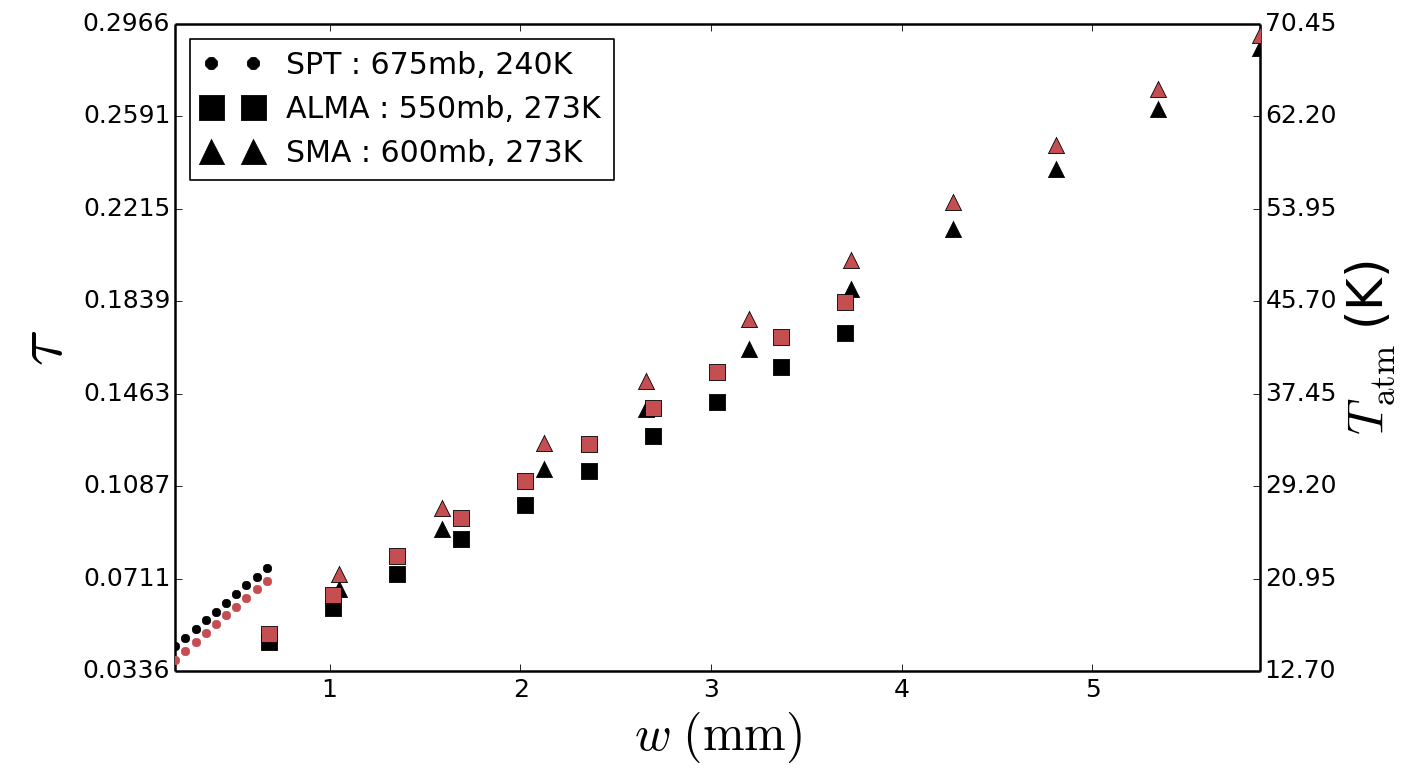
\includegraphics[width=1.\columnwidth]{Images/opacity}
\caption{``Simulated mean opacity (black) and sky brightness temperature (red) at $\nu =230$~GHz  for three typical ground pressures and temperatures over a typical PWV range \citep{Lane_1998} which approximately represent the sites of SPT (dots), ALMA (squares) and SMA (triangles). The legend shows the estimated input ground (pressure, temperature) parameters for each site.''(Image and text reproduced from \citet{Blecher_2016})\label{fig:mean_atm}%
}
\end{figure}


%Turbulent and mean delay
The effects of atmospheric transmission and scattering on delay and delay rate is shown in Fig.~\ref{delay_plots}. The total delay is made up of both mean turbulent components an example of the total and turbulent delays towards Sgr~A* is shown for SMA and ALMA.

\begin{figure}[h!]
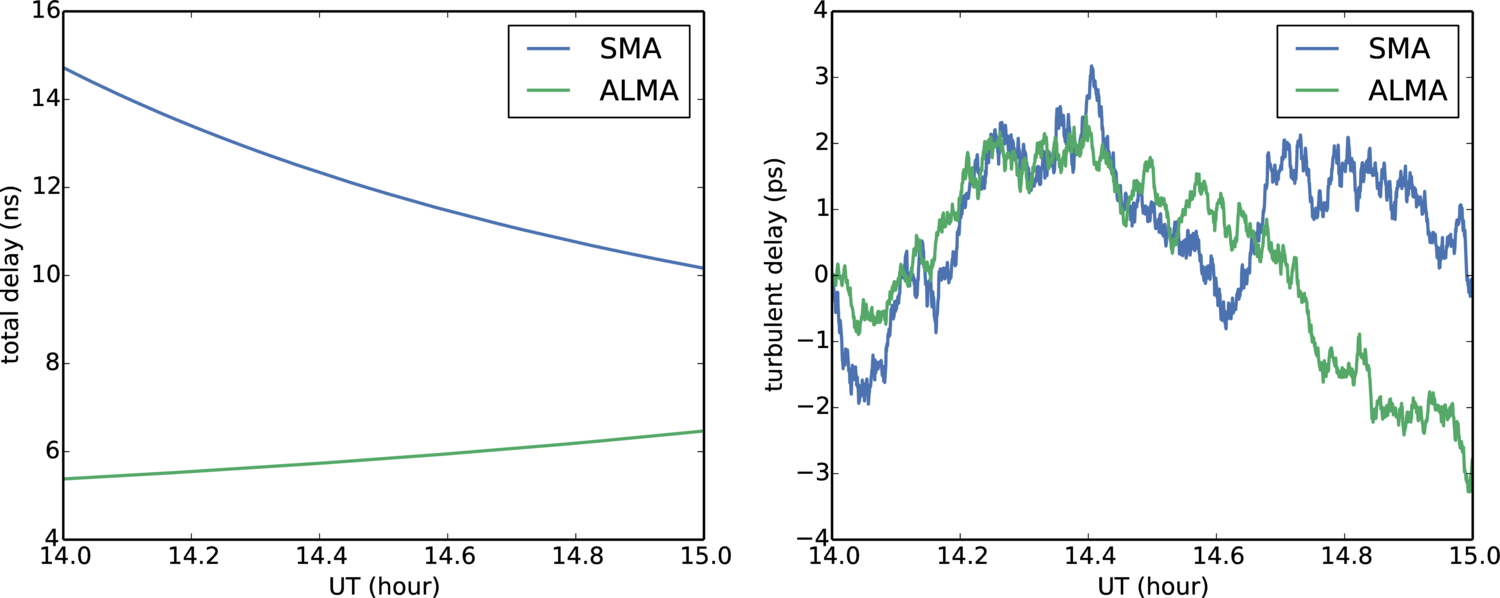
\includegraphics[width=\columnwidth]{Images/delays}
\caption{``Simulation of the total delay (left) and the turbulent atmospheric delay (right) for SMA (blue) and ALMA (green) sites towards Sgr~A$^\star$. Ground pressures and temperatures are the same as Fig.~\ref{fig:mean_atm}, precipitable water vapour above each station is set to $w=2$~mm, and the instantaneous zenith coherence time is set $T_0=10$~s for both stations. Note that all tropospheric parameters are, however, independently set. The conversion from time delay to phase at 230~GHz is $1$~rad~$=0.7$~ps.''(Image and text reproduced from \citet{Blecher_2016})\label{delay_plots}%
}
\end{figure}


%Trop images
``We now investigate the effect of the tropospheric module on image quality for various levels of calibration accuracy. We simulate the simple scenario of a sky model that consists of a 2.4~Jy point source at the phase centre, which is the approximate EHT-measured flux density of Sgr~A$^\star$ at 230~GHz. We assume a zenith phase coherence time of $t_0=10$~s above each station (however, each stations PWV can be independently simulated). We approximate the effect of imperfect calibration by adding a small fraction of the turbulent phase noise. For this example, we do not include the mean delay component, assuming it to be perfectly corrected for during the calibration.''\citep{Blecher_2016}
%Trop images
\begin{figure}[h!]
\includegraphics[width=\columnwidth]{Images/trop_images}
\caption{``The effect of residual troposphere phase noise on interferometric images of a point source observed for 12 hours at 230~GHz with 4~GHz bandwidth with the following array : SPT, ALMA, SMA, SMT, LMT and JCMT, assuming the same SEFDs as \protect\citet{Lu_2014} and an elevation limit of 15$^\circ$. For simplicity the weather parameters at each station were set to: coherence time $t_{\rm 0}=10$~sec; PWV depth $w=1$~mm; ground pressure $P=600$~mb; ground temperature $T =273$~K. {\bf Top left:} interferometric map with thermal noise only. {\bf Top right:} atmospheric attenuation and sky noise (due to non-zero opacity) with 1\% of the turbulent phase noise added. {\bf Bottom left:} as previous but with 3\% of turbulent phase contribution. {\bf Bottom right:} as previous but with 6\% turbulent phase contribution. The fractional turbulent phase contributions are illustrative of the effect of fringe-fitting errors. Note the decrease in the source peak flux with increasing turbulent tropospheric phase noise. Note further that the peak source centroid is offset from its true position (black crosshairs).''(Image and text reproduced from \citet{Blecher_2016}) \label{fig:trop_images}%
}
\end{figure}


%Incoherent closure phases.. This section is needed to link up to the discussion on closure phase uncertainty in the mm-VLBI section




\subsubsection{Pointing}


We investigate the effect of pointing errors on the 50~m (i.e. fully illuminated) Large Millimeter Array (LMT) dish configured in an eight station VLBI array. The LMT has been measured to have an absolute pointing accuracy of $\sigma_{\rm abs} = 1-3$~arcsec, where smaller offsets occur when observing sources closer to zenith, and a tracking pointing accuracy $\sigma_{\rm track} < 1$~arcsec\footnote{http://www.lmtgtm.org/telescope/telescope-description/}. We investigate the observational effect of these errors through three different pointing error models which explore different instructive and plausible scenarios. The LMT has been singled out as this may well serve as a reference station for the EHT array given its sensitivity and central geographic location. The source used is a circular Gaussian of characteristic size $\Theta_{\rm src}=50$ $\mu$-arcsec, located at the phase centre. For this investigation, as long as $\Theta_{\rm src} \ll \theta_{\rm PB}$, the exact structure of the source is unimportant. We approximate the LMT beam profile using an analytic WSRT beam model \citep{Popping_2008} with a factor of two increase in the beam factor $C$ to take into account the increased dish size
\begin{equation}
E(l, m) = \cos^3(C\nu \rho),\qquad   \rho = \sqrt{\delta l_p^2 + \delta m_p^2}
\end{equation}
where $C$ is a constant, with value $C \approx 130$~GHz$^{-1}$. Note that the power beam $EE^H$ becomes $\cos^6$, resulting in a $\rm{FWHM} = 6.5 $~arcsec at 230 GHz. We make use of the RMS fractional visibility amplitude error $\sigma_{\Delta V/V_0}$, where $V_{\rm PE}$ and $V_{0}$ are the visibility amplitudes with and without pointing errors respectively, and  $\Delta V = V_{\rm PE} - V_{0}$ . In Fig.~\ref{fig:pointing}, $\sigma_{\Delta V/V_0}$ is plotted against pointing error $\rho$ over the range $0 \le \rho \le 4.5$~arcsec.

In the first case we assume a \emph{constant} pointing error. This simulation is meant to be instructive as to the typical amplitude error in the simplest possible scenario.



In this simulation, we only consider LMT pointing errors due to its narrow primary beam and potential to be used as a reference station. However, the capability to simulate independent pointing errors for each station is available. In the case of a phased array, a pointing error simulation could be used to investigate the contribution of the pointing error to a variable phasing efficiency, which can be reasonably approximated by a scalar Jones matrix.


\begin{figure}[h!]
\includegraphics[width=\columnwidth]{Images/point_Crop}
\caption{``RMS relative amplitude error induced by pointing error with the 50~m (i.e. fully illuminated) LMT antenna as a function of pointing error offset $\rho$ at 230~GHz. We assume that these errors are degenerate or non-separable from the self-calibration/fringe-fitting model used. See text for the description of the three models used. This simulation capability enables constraints on the magnitude of pointing-induced errors given a particular pointing calibration strategy.''(Image and text reproduced from \citet{Blecher_2016})\label{fig:pointing}%
}
\end{figure}






\section{Calibration and imaging of a time variable source in the presence of the troposphere}
%leave until done
First we fringe fit and image a stationary point source and compare to the result in Fig.~\ref{fig:trop_images}. 


\chapter{Discussion}\label{chap:discussion}

%summary
In section~\ref{sec:sim} we have described the layout of \textsc{MeqSilhouette} synthetic data simulation framework. A wide range of signal propagation effects can be implemented using the Measurement Equation formalism, with tropospheric scattering and antenna pointing errors given as illustrative examples. The framework is sufficiently general and flexible so that time variability in all relevant domains (source, array, ISM, troposphere) can be incorporated. The run time for a typical simulation with a realistic instrumental setup is on the order of minutes.  Implementation of polarisation effects is intended in the next version. 
%link to design objectives
Apparent in these results is the realisation of the design objectives laid out in \ref{sec:des_obj}.

\section{Signal Corruptions}
\subsubsection{ISM}
% Link to diagram in ISM:theory about redoing the Ortiz-leon plot. This is a verification of a large section of the simulator
The reproduction of the \citet{Ortiz_2016} result in Fig.~\ref{fig:substructure2} verifies a large section of the simulation modules, including the interferometric simulation and the ISM simulation module. This also shows the flexibility of the software.

The ISM scattering implementation \textsc{ScatterBrane}, based on \citet*{Johnson_2015a}, has been incorporated into the pipeline. Fig.~\ref{ISM_sequence} provides an example of closure phase and flux variability over a 4 day period using a static source. Accurate simulation of the ISM-induced closure phase variation is essential in order to make any inference on asymmetric, event-horizon scale structure \citep[e.g.][]{Fish_2016,2016arXiv160106571O}. This will become even more important as the EHT sensitivity increases by an order of magnitude in the near future. Note that if the source has intrinsic spatial variability as in the case of a hotspot model \cite{Doeleman_2009}, this will increase ISM variability as the relative motion between source, screen and observer is increased. Furthermore, ISM scattering simulations can constrain the variability fraction associated with the screen, enabling a more robust estimation of source variability, as demonstrated in \citet{Ortiz_2016}.


\subsubsection{Pointing}
In section~\ref{sec:pointing}, we show how antenna pointing errors of the LMT could introduce fractional RMS amplitude variations $\sigma_{\Delta V/V_0} \le 0.4$ on the timescale of phase centre switching. This would occur if the calibrator is widely separated from the source, as is often the case in mm-VLBI. In contrast tracking errors are less problematic with $\sigma_{\Delta V/V_0} \le 0.05$. If the gain error is non-separable from the calibration model used, it could be interpreted as intrinsic variability, substructure and/or increased noise. If unaccounted for, this effect has the potential to limit the dynamic range of mm-VLBI images. Further tests to constrain the pointing uncertainties of EHT stations will lead to more accurate interferometric simulations and hence the overall impact on black hole shadow parameter estimation. Here we demonstrate the capability to incorporate a range of plausible pointing error effects into a full simulation pipeline.  

Visibility amplitude errors due to antenna pointing error has been investigated for the $50$~m  LMT dish operating at $230$~GHz. In Fig.~\ref{fig:pointing}, we show that pointing errors associated with frequent phase centre switching (stochastic variability) could introduce a RMS fractional amplitude error $\sigma_{\Delta V/V_0} \sim 0.1 - 0.4$ for an absolute pointing accuracy  $\sigma_{\rm abs} \sim 1-3$~arcsec. In contrast, tracking errors are less problematic with $\sigma_{\Delta V/V_0} \le 0.05$ for a tracking accuracy  $\sigma_{\rm track}<1$~arcsec. The case of a constant error pointing model is comparable to that of the `slow variability' case. If the gain error is non-separable from the calibration model used, it could be interpreted as intrinsic variability, substructure and/or increased noise. If unaccounted for, this effect has the potential to limit the dynamic range of mm-VLBI images. Further tests to constrain the pointing uncertainties of EHT stations will lead to more accurate interferometric simulations and hence the overall impact on black hole shadow parameter estimation. Here we demonstrate the capability to incorporate a range of plausible pointing error effects into a full simulation pipeline. For future observations at 345~GHz, these effects will be even more pronounced, given the narrower primary beam. 


\subsubsection{Trop} 
``In Fig.~\ref{fig:trop_images} we explore the observational consequences of observing through a turbulent troposphere. In this simulation, we assume a simple point source model and apply increasing levels of turbulence-induced phase fluctuations before imaging using the two dimensional inverse fast Fourier transforms. We note a rapid attenuation in peak flux due to incoherent averaging, slight offsets in the source centroid and the presence of spurious imaging artefacts. Suprisingly, in this configuration, there was no evidence of blurring or a loss of resolution with the uncertainties. In an upcoming paper, we perform a systematic exploration of the turbulent tropospheric effects on the accuracy of fringe-fitting algorithms/strategies, through use of an automated calibration procedure and including the added complexity of a time-variable source.''\citep{Blecher_2016


Significant progress has been made in the theoretical and numerical modeling of the inner accretion flow and jet launch regions near a supermassive black hole event horizon
\citep[e.g.][]{Zanna_2007,Etienne_2010,Dexter_2013,Moscibrodzka_2014, McKinney_2014}. As the sensitivity of the EHT stands to dramatically increase, these theoretical efforts must be complemented by advances in interferometric simulations. With \textsc{MeqSilhouette}, we now have the ability to couple these with sophisticated interferometric and signal propagation simulations.  Moreover, detailed interferometric simulations will enable us to quantify systematic effects on the black hole and/or accretion flow parameter estimation.



NON-CLOSING ERRORS
Non-closing errors due to incoherent averaging - "no conjugates for triples" - possibly comes down to how one defines SNR. In the definition used in the literature we followed, they assumed only gaussian noise, which was not the case..A better definition would be to look at the distribution of a number of samples 


Why no seeing? - seeing results when the decoherence is considered as a function of baseline length, longer baseline are more decoherent and their visibilities are downweighted. For the EHT as different stations would experience independent different turbulent intensities, the baseline length will not be correlated with the magnitude of the seeing. But this will still distort the image, leading to uncharacteristic feature extraction....ummm taken the blurring sentence out of the paper on roger's instruction


\section{Suggested future improvements to the simulator}

\subsection{Full Stokes}

Later versions of {\sc MeqSilhouette} will enable the full Stokes cubes as input. This should not entail much work as our chosen data formats (MS, {\sc fits}) and the simulator in {\sc MeqTrees} already support full stokes logic. Signal propagation through the ISM and troposphere as well as antenna based complex gains errors are polarisation independent. The work would be primarly involve altering the existing scripts to dealing with the extra dimension in the {\sc fits} files i.e. book keeping. 
polarisation leakage in the RIME.

\subsection{Opacity and atmospheric brightness temperature fluctuations}

Run multiple realisations of atm to link the phase fluctuations to opacity and brightness temperature fluctuations possibly by fluctuating the input climate parameters., but this might be unfeasible.




